\section{Allgemein}

\textbf{Mitternachtsformel}

\[
    x_{1, 2} = \frac{-b \pm \sqrt{b^2 - 4ac}}{2a}
\]

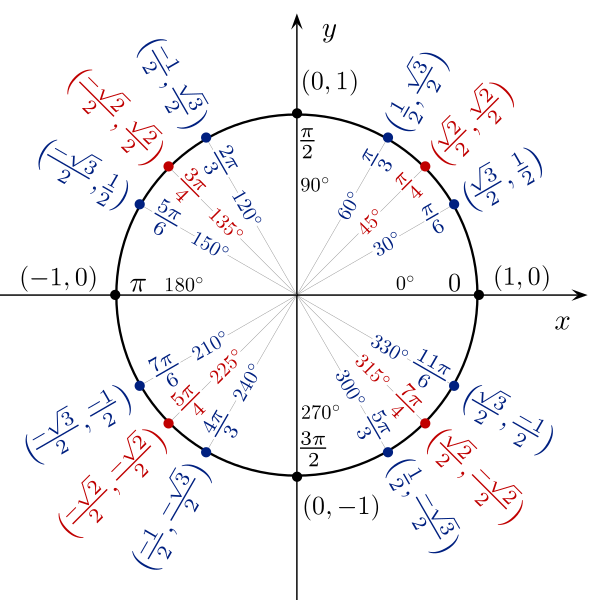
\includegraphics[width=7cm]{angles}

\textbf{Matrix Determinante}

\[
    \begin{vmatrix}
        a & b\\
        c & d
    \end{vmatrix} = ad-bc
\]

\textbf{Matrix Invertierbarkeit}: Eine quadratische Matrix ist genau dann invertierbar, falls die Determinante $\neq 0$.

\textbf{Matrix positiv definit}: Alle Eigenwerte $\lambda_1, ..., \lambda_n > 0$, \textbf{negativ definit:} Alle Eigenwerte $\lambda_1, ..., \lambda_n < 0$, \textbf{indefinit:} Eigenwerte sind positiv und negativ.\\

\textbf{Skalarprodukt} \[ x \cdot y = \sum_{i=1}^n x_i y_i \]